

\tikzset{every picture/.style={line width=0.75pt}} %set default line width to 0.75pt        

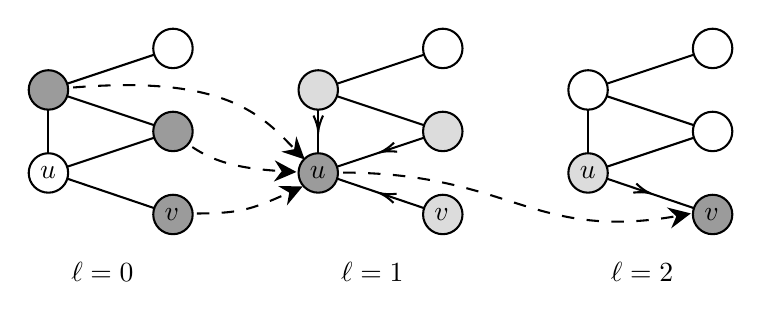
\begin{tikzpicture}[x=0.75pt,y=0.75pt,yscale=-1,xscale=1]
%uncomment if require: \path (0,160); %set diagram left start at 0, and has height of 160

%Curve Lines [id:da4313717085077018] 
\draw  [dash pattern={on 4.5pt off 4.5pt}]  (40.5,40.5) .. controls (128.99,30.61) and (144.66,54.47) .. (162.09,72.11) ;
\draw [shift={(164,74)}, rotate = 224.13] [fill={rgb, 255:red, 0; green, 0; blue, 0 }  ][line width=0.08]  [draw opacity=0] (10.72,-5.15) -- (0,0) -- (10.72,5.15) -- (7.12,0) -- cycle    ;
%Curve Lines [id:da6954216550236572] 
\draw  [dash pattern={on 4.5pt off 4.5pt}]  (100.5,60.5) .. controls (116.13,75.22) and (130.65,78.52) .. (157.08,79.86) ;
\draw [shift={(160,80)}, rotate = 182.53] [fill={rgb, 255:red, 0; green, 0; blue, 0 }  ][line width=0.08]  [draw opacity=0] (10.72,-5.15) -- (0,0) -- (10.72,5.15) -- (7.12,0) -- cycle    ;
%Curve Lines [id:da3347980352129689] 
\draw  [dash pattern={on 4.5pt off 4.5pt}]  (100,100) .. controls (132.69,100.24) and (135.08,99.78) .. (160.57,88.11) ;
\draw [shift={(163,87)}, rotate = 515.36] [fill={rgb, 255:red, 0; green, 0; blue, 0 }  ][line width=0.08]  [draw opacity=0] (10.72,-5.15) -- (0,0) -- (10.72,5.15) -- (7.12,0) -- cycle    ;
%Curve Lines [id:da07095702036161233] 
\draw  [dash pattern={on 4.5pt off 4.5pt}]  (170.5,80.5) .. controls (264.25,77.28) and (270.58,115.47) .. (347.64,100.47) ;
\draw [shift={(350,100)}, rotate = 528.4200000000001] [fill={rgb, 255:red, 0; green, 0; blue, 0 }  ][line width=0.08]  [draw opacity=0] (10.72,-5.15) -- (0,0) -- (10.72,5.15) -- (7.12,0) -- cycle    ;
%Straight Lines [id:da47912352597118213] 
\draw    (40.5,50) -- (40.5,71) ;
%Straight Lines [id:da9922159879153771] 
\draw    (40.5,40.5) -- (100.5,60.5) ;
%Straight Lines [id:da20693867709022928] 
\draw    (40.5,80.5) -- (100.5,60.5) ;
%Straight Lines [id:da12726884670105187] 
\draw    (40,80) -- (100.5,100.5) ;
%Straight Lines [id:da005529487369804631] 
\draw    (100.5,20.5) -- (40.5,40.5) ;
%Shape: Circle [id:dp12978240920475836] 
\draw  [fill={rgb, 255:red, 155; green, 155; blue, 155 }  ,fill opacity=1 ] (31,40.5) .. controls (31,35.25) and (35.25,31) .. (40.5,31) .. controls (45.75,31) and (50,35.25) .. (50,40.5) .. controls (50,45.75) and (45.75,50) .. (40.5,50) .. controls (35.25,50) and (31,45.75) .. (31,40.5) -- cycle ;
%Shape: Circle [id:dp44461896764010267] 
\draw  [fill={rgb, 255:red, 255; green, 255; blue, 255 }  ,fill opacity=1 ] (91,20.5) .. controls (91,15.25) and (95.25,11) .. (100.5,11) .. controls (105.75,11) and (110,15.25) .. (110,20.5) .. controls (110,25.75) and (105.75,30) .. (100.5,30) .. controls (95.25,30) and (91,25.75) .. (91,20.5) -- cycle ;
%Shape: Circle [id:dp8226342601300562] 
\draw  [fill={rgb, 255:red, 155; green, 155; blue, 155 }  ,fill opacity=1 ] (91,60.5) .. controls (91,55.25) and (95.25,51) .. (100.5,51) .. controls (105.75,51) and (110,55.25) .. (110,60.5) .. controls (110,65.75) and (105.75,70) .. (100.5,70) .. controls (95.25,70) and (91,65.75) .. (91,60.5) -- cycle ;
%Shape: Circle [id:dp9576590983310105] 
\draw  [fill={rgb, 255:red, 255; green, 255; blue, 255 }  ,fill opacity=1 ] (31,80.5) .. controls (31,75.25) and (35.25,71) .. (40.5,71) .. controls (45.75,71) and (50,75.25) .. (50,80.5) .. controls (50,85.75) and (45.75,90) .. (40.5,90) .. controls (35.25,90) and (31,85.75) .. (31,80.5) -- cycle ;
%Shape: Circle [id:dp6767076773328078] 
\draw  [fill={rgb, 255:red, 155; green, 155; blue, 155 }  ,fill opacity=1 ] (91,100.5) .. controls (91,95.25) and (95.25,91) .. (100.5,91) .. controls (105.75,91) and (110,95.25) .. (110,100.5) .. controls (110,105.75) and (105.75,110) .. (100.5,110) .. controls (95.25,110) and (91,105.75) .. (91,100.5) -- cycle ;
%Straight Lines [id:da3797310936600804] 
\draw    (170.5,50) -- (170.5,71) ;
\draw [shift={(170.5,60.5)}, rotate = 270] [color={rgb, 255:red, 0; green, 0; blue, 0 }  ][line width=0.75]    (7.65,-2.3) .. controls (4.86,-0.97) and (2.31,-0.21) .. (0,0) .. controls (2.31,0.21) and (4.86,0.98) .. (7.65,2.3)   ;
%Straight Lines [id:da39313117597338243] 
\draw    (170.5,40.5) -- (230.5,60.5) ;
%Straight Lines [id:da11909283508234703] 
\draw    (170.5,80.5) -- (230.5,60.5) ;
\draw [shift={(200.5,70.5)}, rotate = 341.57] [color={rgb, 255:red, 0; green, 0; blue, 0 }  ][line width=0.75]    (7.65,-2.3) .. controls (4.86,-0.97) and (2.31,-0.21) .. (0,0) .. controls (2.31,0.21) and (4.86,0.98) .. (7.65,2.3)   ;
%Straight Lines [id:da3511148855222339] 
\draw    (170,80) -- (230.5,100.5) ;
\draw [shift={(200.25,90.25)}, rotate = 18.72] [color={rgb, 255:red, 0; green, 0; blue, 0 }  ][line width=0.75]    (7.65,-2.3) .. controls (4.86,-0.97) and (2.31,-0.21) .. (0,0) .. controls (2.31,0.21) and (4.86,0.98) .. (7.65,2.3)   ;
%Straight Lines [id:da6106293032869707] 
\draw    (230.5,20.5) -- (170.5,40.5) ;
%Shape: Circle [id:dp4701031138690044] 
\draw  [fill={rgb, 255:red, 220; green, 220; blue, 220 }  ,fill opacity=1 ] (161,40.5) .. controls (161,35.25) and (165.25,31) .. (170.5,31) .. controls (175.75,31) and (180,35.25) .. (180,40.5) .. controls (180,45.75) and (175.75,50) .. (170.5,50) .. controls (165.25,50) and (161,45.75) .. (161,40.5) -- cycle ;
%Shape: Circle [id:dp5321807173132955] 
\draw  [fill={rgb, 255:red, 255; green, 255; blue, 255 }  ,fill opacity=1 ] (221,20.5) .. controls (221,15.25) and (225.25,11) .. (230.5,11) .. controls (235.75,11) and (240,15.25) .. (240,20.5) .. controls (240,25.75) and (235.75,30) .. (230.5,30) .. controls (225.25,30) and (221,25.75) .. (221,20.5) -- cycle ;
%Shape: Circle [id:dp554517566024453] 
\draw  [fill={rgb, 255:red, 220; green, 220; blue, 220 }  ,fill opacity=1 ] (221,60.5) .. controls (221,55.25) and (225.25,51) .. (230.5,51) .. controls (235.75,51) and (240,55.25) .. (240,60.5) .. controls (240,65.75) and (235.75,70) .. (230.5,70) .. controls (225.25,70) and (221,65.75) .. (221,60.5) -- cycle ;
%Shape: Circle [id:dp6234497550508977] 
\draw  [fill={rgb, 255:red, 155; green, 155; blue, 155 }  ,fill opacity=1 ] (161,80.5) .. controls (161,75.25) and (165.25,71) .. (170.5,71) .. controls (175.75,71) and (180,75.25) .. (180,80.5) .. controls (180,85.75) and (175.75,90) .. (170.5,90) .. controls (165.25,90) and (161,85.75) .. (161,80.5) -- cycle ;
%Shape: Circle [id:dp6481128593514689] 
\draw  [fill={rgb, 255:red, 220; green, 220; blue, 220 }  ,fill opacity=1 ] (221,100.5) .. controls (221,95.25) and (225.25,91) .. (230.5,91) .. controls (235.75,91) and (240,95.25) .. (240,100.5) .. controls (240,105.75) and (235.75,110) .. (230.5,110) .. controls (225.25,110) and (221,105.75) .. (221,100.5) -- cycle ;
%Straight Lines [id:da010045754906601312] 
\draw    (300.5,50) -- (300.5,71) ;
%Straight Lines [id:da9723039406561984] 
\draw    (300.5,40.5) -- (360.5,60.5) ;
%Straight Lines [id:da7207693173524592] 
\draw    (300.5,80.5) -- (360.5,60.5) ;
%Straight Lines [id:da047867810436508895] 
\draw    (300,80) -- (360.5,100.5) ;
\draw [shift={(330.25,90.25)}, rotate = 198.72] [color={rgb, 255:red, 0; green, 0; blue, 0 }  ][line width=0.75]    (7.65,-2.3) .. controls (4.86,-0.97) and (2.31,-0.21) .. (0,0) .. controls (2.31,0.21) and (4.86,0.98) .. (7.65,2.3)   ;
%Straight Lines [id:da13877434621766804] 
\draw    (360.5,20.5) -- (300.5,40.5) ;
%Shape: Circle [id:dp9753163859311793] 
\draw  [fill={rgb, 255:red, 255; green, 255; blue, 255 }  ,fill opacity=1 ] (291,40.5) .. controls (291,35.25) and (295.25,31) .. (300.5,31) .. controls (305.75,31) and (310,35.25) .. (310,40.5) .. controls (310,45.75) and (305.75,50) .. (300.5,50) .. controls (295.25,50) and (291,45.75) .. (291,40.5) -- cycle ;
%Shape: Circle [id:dp03916750111680778] 
\draw  [fill={rgb, 255:red, 255; green, 255; blue, 255 }  ,fill opacity=1 ] (351,20.5) .. controls (351,15.25) and (355.25,11) .. (360.5,11) .. controls (365.75,11) and (370,15.25) .. (370,20.5) .. controls (370,25.75) and (365.75,30) .. (360.5,30) .. controls (355.25,30) and (351,25.75) .. (351,20.5) -- cycle ;
%Shape: Circle [id:dp7074039311567142] 
\draw  [fill={rgb, 255:red, 255; green, 255; blue, 255 }  ,fill opacity=1 ] (351,60.5) .. controls (351,55.25) and (355.25,51) .. (360.5,51) .. controls (365.75,51) and (370,55.25) .. (370,60.5) .. controls (370,65.75) and (365.75,70) .. (360.5,70) .. controls (355.25,70) and (351,65.75) .. (351,60.5) -- cycle ;
%Shape: Circle [id:dp4904701423686293] 
\draw  [fill={rgb, 255:red, 220; green, 220; blue, 220 }  ,fill opacity=1 ] (291,80.5) .. controls (291,75.25) and (295.25,71) .. (300.5,71) .. controls (305.75,71) and (310,75.25) .. (310,80.5) .. controls (310,85.75) and (305.75,90) .. (300.5,90) .. controls (295.25,90) and (291,85.75) .. (291,80.5) -- cycle ;
%Shape: Circle [id:dp8890572986824241] 
\draw  [fill={rgb, 255:red, 155; green, 155; blue, 155 }  ,fill opacity=1 ] (351,100.5) .. controls (351,95.25) and (355.25,91) .. (360.5,91) .. controls (365.75,91) and (370,95.25) .. (370,100.5) .. controls (370,105.75) and (365.75,110) .. (360.5,110) .. controls (355.25,110) and (351,105.75) .. (351,100.5) -- cycle ;

% Text Node
\draw (355,96) node [anchor=north west][inner sep=0.75pt]    {$v$};
% Text Node
\draw (225,96) node [anchor=north west][inner sep=0.75pt]    {$v$};
% Text Node
\draw (95,96) node [anchor=north west][inner sep=0.75pt]    {$v$};
% Text Node
\draw (295,76) node [anchor=north west][inner sep=0.75pt]    {$u$};
% Text Node
\draw (165,76) node [anchor=north west][inner sep=0.75pt]    {$u$};
% Text Node
\draw (35,76) node [anchor=north west][inner sep=0.75pt]    {$u$};

% Text Node
\draw (50,122) node [anchor=north west][inner sep=0.75pt]    {$\ell =0$};
% Text Node
\draw (180,122) node [anchor=north west][inner sep=0.75pt]    {$\ell =1$};
% Text Node
\draw (310,122) node [anchor=north west][inner sep=0.75pt]    {$\ell =2$};


\end{tikzpicture}